% Diagram: Transformer Layer Architecture and GPU Memory Layout
% Used in: Chapter 4, Section 4.1 (How Architecture Connects to Weights)
\begin{figure}[htbp]
\centering
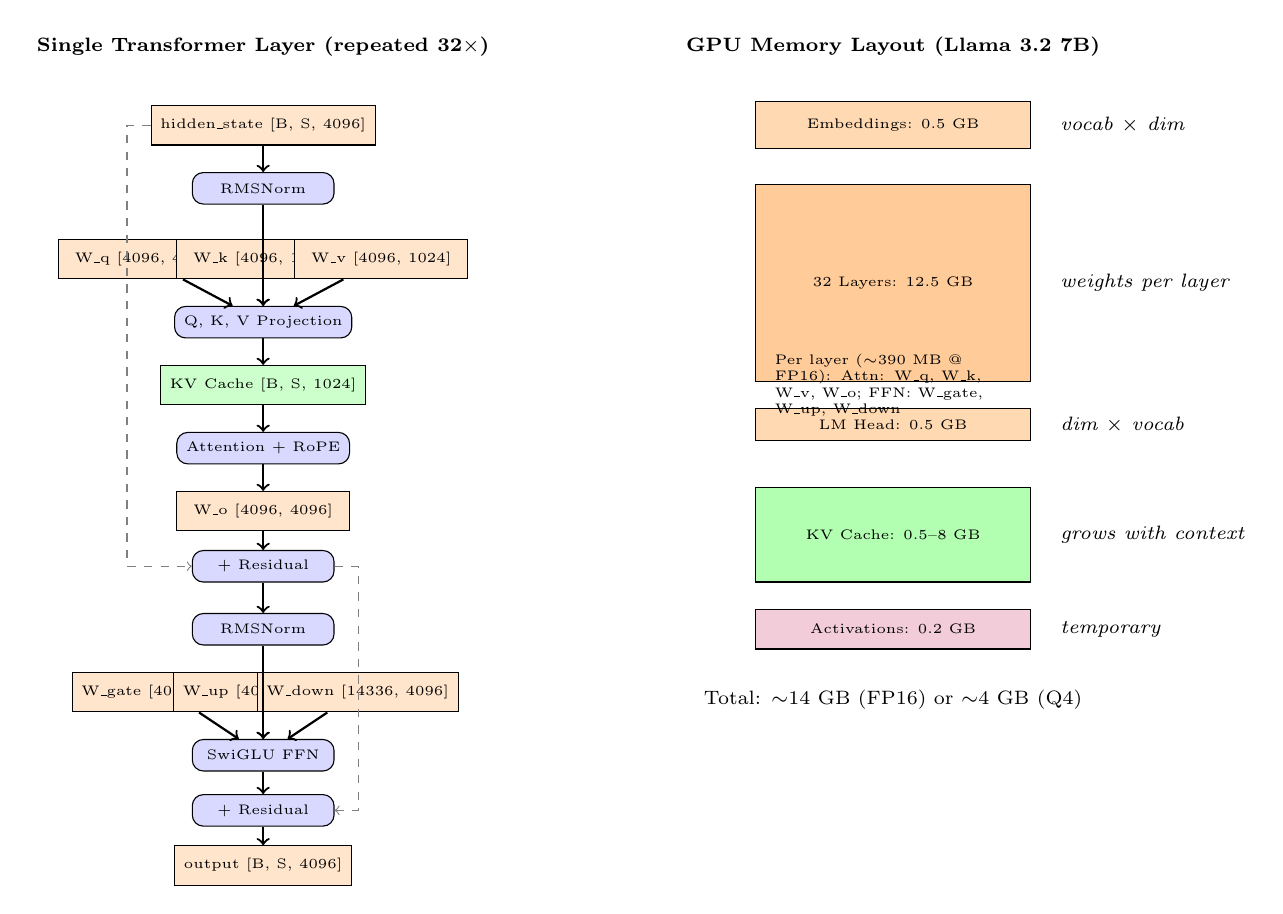
\begin{tikzpicture}[
    node distance=0.4cm,
    tensor/.style={rectangle, draw, minimum width=2.2cm, minimum height=0.5cm, font=\tiny, fill=orange!20},
    operation/.style={rectangle, draw, rounded corners, minimum width=1.8cm, minimum height=0.4cm, font=\tiny, fill=blue!15},
    cache/.style={rectangle, draw, minimum width=2.2cm, minimum height=0.5cm, font=\tiny, fill=green!20},
    arrow/.style={->, thick},
    label/.style={font=\scriptsize}
]

% === LEFT SIDE: Single Transformer Layer ===
\node[label] at (-4, 4.5) {\textbf{Single Transformer Layer (repeated 32$\times$)}};

% Input
\node[tensor] (input) at (-4, 3.5) {hidden\_state [B, S, 4096]};

% Attention block
\node[operation] (attn_norm) at (-4, 2.7) {RMSNorm};
\node[tensor] (wq) at (-5.5, 1.8) {W\_q [4096, 4096]};
\node[tensor] (wk) at (-4, 1.8) {W\_k [4096, 1024]};
\node[tensor] (wv) at (-2.5, 1.8) {W\_v [4096, 1024]};
\node[operation] (qkv) at (-4, 1.0) {Q, K, V Projection};
\node[cache] (kvcache) at (-4, 0.2) {KV Cache [B, S, 1024]};
\node[operation] (attn) at (-4, -0.6) {Attention + RoPE};
\node[tensor] (wo) at (-4, -1.4) {W\_o [4096, 4096]};
\node[operation] (add1) at (-4, -2.1) {+ Residual};

% FFN block
\node[operation] (ffn_norm) at (-4, -2.9) {RMSNorm};
\node[tensor] (wgate) at (-5.2, -3.7) {W\_gate [4096, 14336]};
\node[tensor] (wup) at (-4, -3.7) {W\_up [4096, 14336]};
\node[tensor] (wdown) at (-2.8, -3.7) {W\_down [14336, 4096]};
\node[operation] (ffn) at (-4, -4.5) {SwiGLU FFN};
\node[operation] (add2) at (-4, -5.2) {+ Residual};
\node[tensor] (output) at (-4, -5.9) {output [B, S, 4096]};

% Arrows for left side
\draw[arrow] (input) -- (attn_norm);
\draw[arrow] (attn_norm) -- (qkv);
\draw[arrow] (wq) -- (qkv);
\draw[arrow] (wk) -- (qkv);
\draw[arrow] (wv) -- (qkv);
\draw[arrow] (qkv) -- (kvcache);
\draw[arrow] (kvcache) -- (attn);
\draw[arrow] (attn) -- (wo);
\draw[arrow] (wo) -- (add1);
\draw[arrow] (add1) -- (ffn_norm);
\draw[arrow] (ffn_norm) -- (ffn);
\draw[arrow] (wgate) -- (ffn);
\draw[arrow] (wup) -- (ffn);
\draw[arrow] (wdown) -- (ffn);
\draw[arrow] (ffn) -- (add2);
\draw[arrow] (add2) -- (output);

% Residual connections
\draw[->, dashed, gray] (input.west) -- ++(-0.3,0) |- (add1.west);
\draw[->, dashed, gray] (add1.east) -- ++(0.3,0) |- (add2.east);

% === RIGHT SIDE: GPU Memory Layout ===
\node[label] at (4, 4.5) {\textbf{GPU Memory Layout (Llama 3.2 7B)}};

% Memory blocks
\node[tensor, minimum width=3.5cm, minimum height=0.6cm, fill=orange!30] (emb) at (4, 3.5) {Embeddings: 0.5 GB};
\node[tensor, minimum width=3.5cm, minimum height=2.5cm, fill=orange!40] (layers) at (4, 1.5) {32 Layers: 12.5 GB};
\node[tensor, minimum width=3.5cm, minimum height=0.4cm, fill=orange!30] (head) at (4, -0.3) {LM Head: 0.5 GB};
\node[cache, minimum width=3.5cm, minimum height=1.2cm, fill=green!30] (kv) at (4, -1.7) {KV Cache: 0.5--8 GB};
\node[tensor, minimum width=3.5cm, minimum height=0.5cm, fill=purple!20] (act) at (4, -2.9) {Activations: 0.2 GB};

% Memory size annotations
\node[label, right] at (6, 3.5) {\textit{vocab $\times$ dim}};
\node[label, right] at (6, 1.5) {\textit{weights per layer}};
\node[label, right] at (6, -0.3) {\textit{dim $\times$ vocab}};
\node[label, right] at (6, -1.7) {\textit{grows with context}};
\node[label, right] at (6, -2.9) {\textit{temporary}};

% Total
\node[label] at (4, -3.8) {Total: $\sim$14 GB (FP16) or $\sim$4 GB (Q4)};

% Per-layer breakdown
\node[label, align=left, font=\tiny, text width=3cm] at (4, 0.2) {
Per layer ($\sim$390 MB @ FP16):
Attn: W\_q, W\_k, W\_v, W\_o;
FFN: W\_gate, W\_up, W\_down
};

\end{tikzpicture}
\caption{Left: computation flow through one transformer layer with weight tensors (orange) and KV cache (green). Right: GPU memory layout for Llama 3.2 7B showing how weights, cache, and activations occupy VRAM.}
\label{fig:transformer-memory-layout}
\end{figure}
